\chapter{Разработка систем компьютерного зрения на основе глубоких нейронных сетей}

Научные и практические результаты, полученные в рамках данной диссертационной работы, внедрены и используются на следующих предприятиях Республики Беларусь:

\begin{easylist}
	& <<Intelligent Semantic Systems>> (г. Минск) при разработке подсистемы компьютерного зрения для осуществления распознавания объектов;
	& ОАО <<Савушкин продукт>> (г. Брест) при разработке системы автоматического контроля качества нанесения маркировки продукции;
	& в учебном процессе учреждения образования <<Брестский государственный технический университет>>.
 \end{easylist}

Сведения об использовании результатов диссертационной работы отражены в соответствующих актах внедрения, приведенных в приложении \ref{app:b}.

\section{Обнаружение солнечных панелей на аэрофотоснимках}

\subsection{Постановка задачи и обзор существующих решений}
По причине увеличивающейся доли использования солнечной энергии, спрос на фотоэлектрические элементы в мире постоянно растет. С начала 2010-х годов индустрия производства и поддержки солнечных панелей переживает стремительный рост. Так, по состоянию на 2022 год только в США в данной отрасли работает более 10000 компаний и 263.000 сотрудников \cite{seia}.

В связи с растущей популярностью этой технологии проблемы, связанные с обслуживанием солнечных панелей, также становятся актуальными. Многие сервисные компании заинтересованы в получении информации о потенциальных клиентах. Таким образом, анализ фотоснимков с целью обнаружения солнечных панелей и накопления статистической информации является актуальной задачей.

%Развитие теории обучения глубоких нейронных сетей [4] дало мощный импульс для разработки различных вариантов сверточных нейронных сетей, применяемых для решения задач распознавания и классификации. Появление технологии параллелизации вычислений с использованием GPU в свою очередь сделало такое обучение осуществимым за приемлемый отрезок времени.

Поставленная задача заключалась в разработке системы обнаружения солнечных панелей на изображениях с их последующей локализацией.

В статье Дж. Малофа \cite{malof2015} был описан подход, базирующийся на использовании SVM для автоматического обнаружения солнечных панелей, используя фотографии высокого разрешения, полученные с помощью спутника. В этом подходе сначала применяется операция предварительного скрининга, которая идентифицирует регионы, которые затем обрабатываются с целью выделения признаков. В качестве выходной информации, получаемой с помощью данной модели, выступает список регионов и доверительные значения, показывающие, насколько вероятно наличие солнечной панели в заданной области. Общая эффективность подхода определения наличия панелей в \cite{malof2015} составляет порядка 94\%. Однако, нужно отметить, что данный метод дает лишь приблизительную информацию о местонахождении панели. Оценки точности локализации панелей в работе не приводится.

В \cite{malof2016} используется подход, базирующийся на применении деревьев решений. Достигнутый показатель локализации панелей составил 90\% в случае использования определенных параметров алгоритма, а сам метод состоит из четырех стадий. В работе в качестве обучающей выборки используется Aerial Imagery Dataset, включающий изображения разрешением до 5000 Х 5000 пикселей \cite{bradbury2016}.

\subsection{Предлагаемый подход}

Предложенный нейросетевой алгоритм для обнаружения солнечных панелей отличается тем, что в качестве базовой модели используется сверточная нейронная сеть, которая показывает лучшие результаты при решении задач классификации и детекции объектов на изображениях. Другое важное отличие заключается в использовании фотографий низкого разрешения для обучения нашей модели (например, фото из Google Maps, нередко неудовлетворительного качества, рисунок \ref{fig:example_of_images}). 

\begin{figure}[ht]
	\centering
	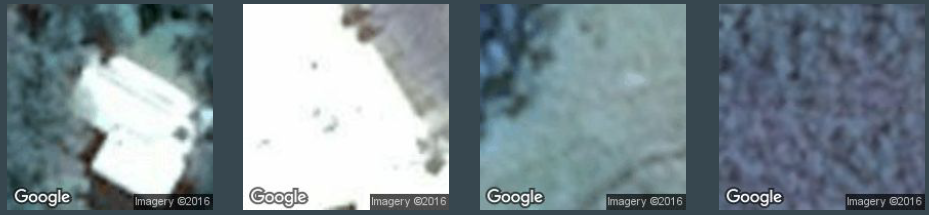
\includegraphics[width=16cm]{man-source/images/ch4/pic4-16.png}
	\caption{Примеры изображений низкого качества из обучающей выборки}
	\label{fig:example_of_images}
\end{figure}

Предлагаемая система обнаружения солнечных панелей включает два основных компонента, в составе которых используются предобученные глубокие нейронные сети: 

\begin{easylistNum}
    & классификатор для оценки наличия солнечной панели на аэрофотоснимке;
    & детектор для локализации солнечной панели (рисунок \ref{fig:solar_system_arch}).
\end{easylistNum}

\begin{figure}[ht]
	\centering
	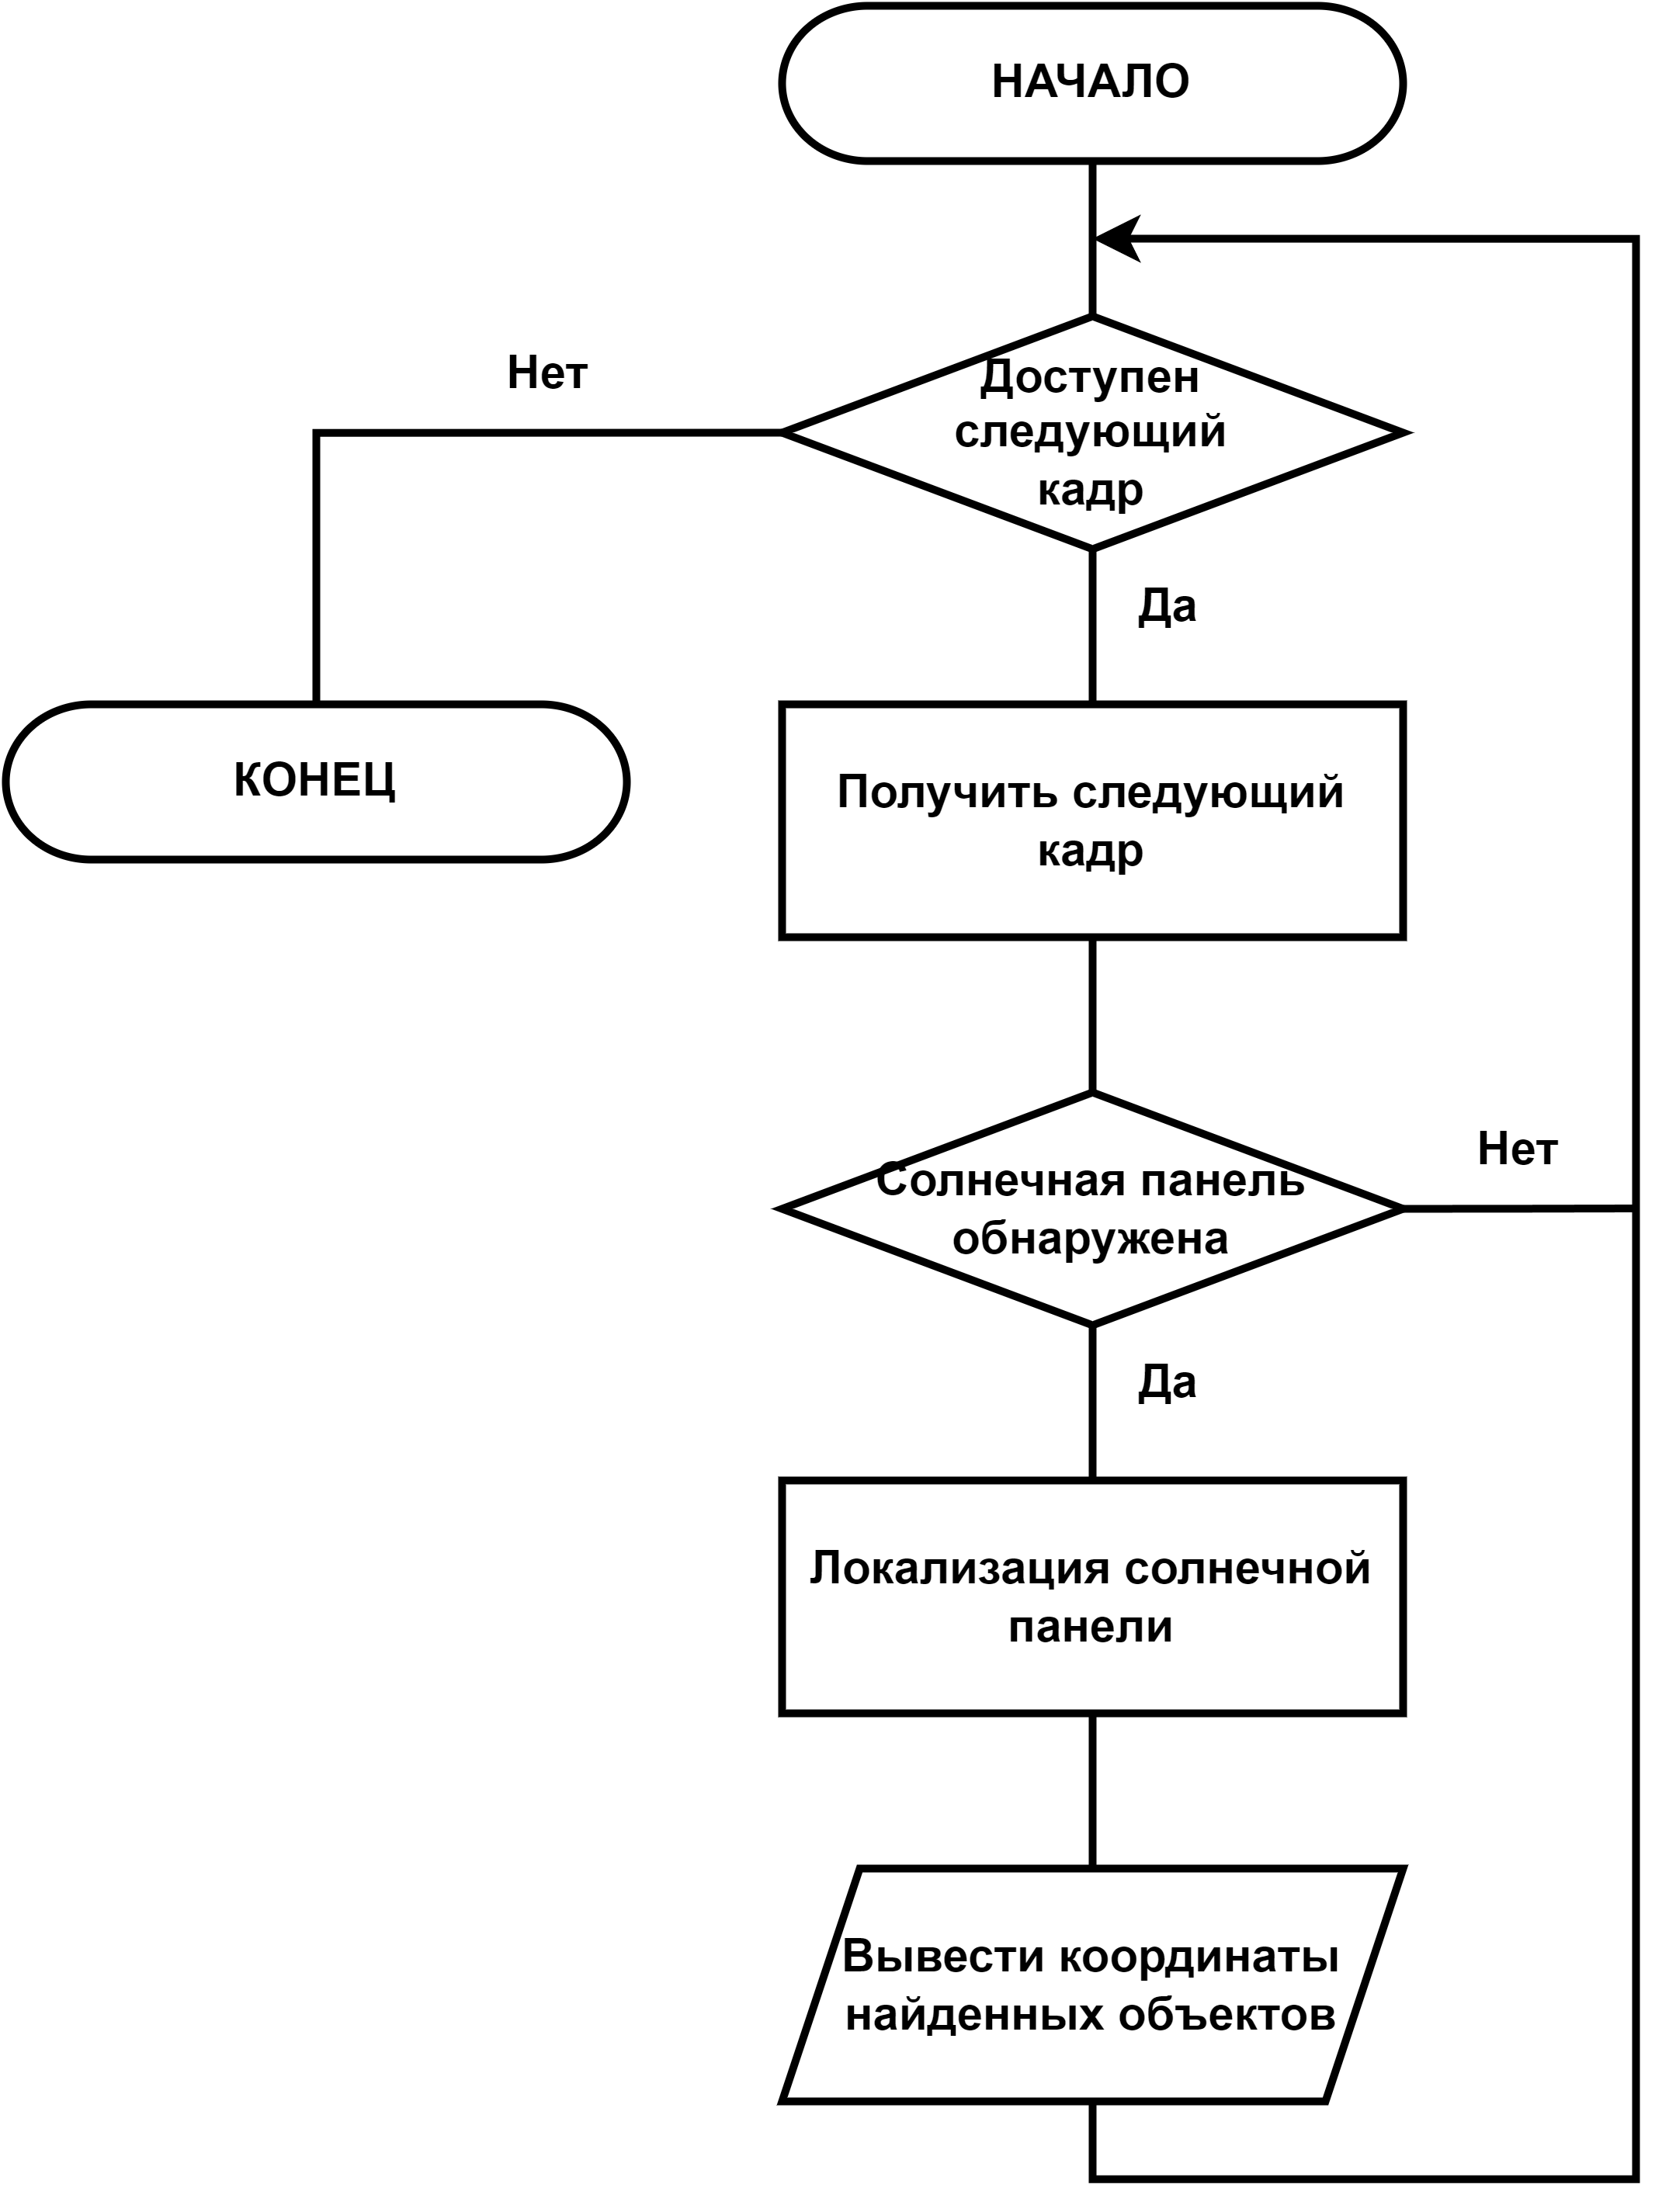
\includegraphics[width=12cm]{man-source/images/ch4/pic4-16a.png}
	\caption{Блок-схема работы системы обнаружения солнечных панелей}
	\label{fig:solar_system_arch}
\end{figure}

Двухэтапность в решении поставленной задачи позволяет существенно ускорить обработку изображений, большую часть которых занимают объекты, отличные от искомых (солнечных панелей), т.к. нейросетевые модели, используемые на этапе локализации, как правило, более ресурсоемки. Таким образом, модель первого этапа выполняет роль фильтра для последующей обработки. Тем самым предлагаемый алгоритм можно применять для последовательной обработки больших изображений.

\textbf{Классификатор для оценки наличия солнечной панели на аэрофотоснимке}. Для этой подзадачи применялся сверточный классификатор с архитектурой, представленной на рисунке \ref{fig:used_cnn} [35]. 

\begin{figure}[ht]
	\centering
	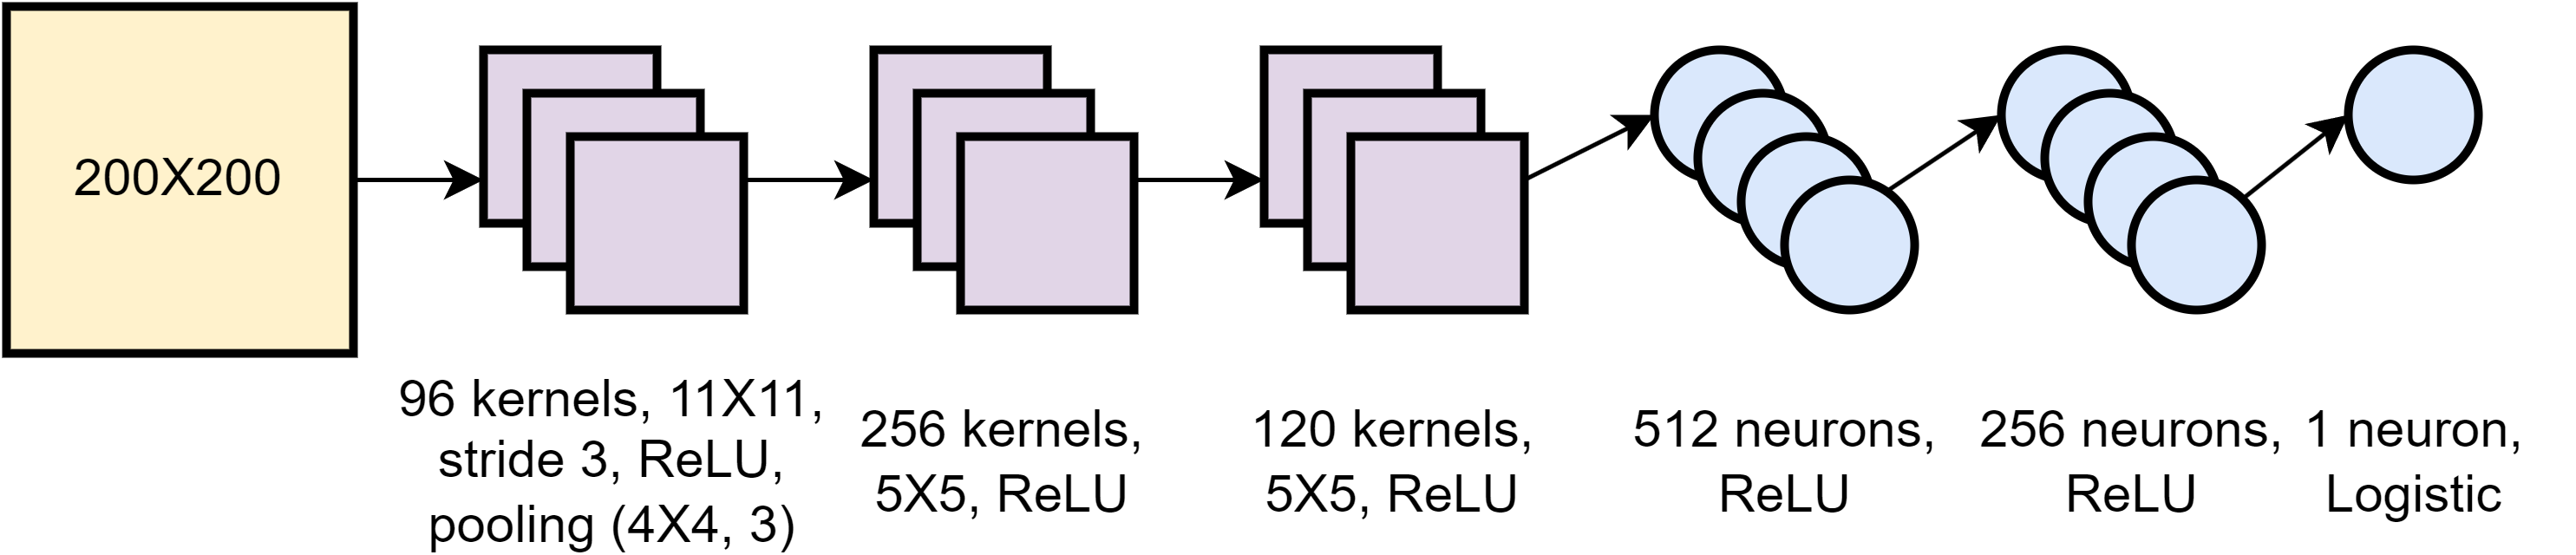
\includegraphics[width=17cm]{man-source/images/ch4/pic4-19.png}
	\caption{Архитектура используемой сверточной нейронной сети}
	\label{fig:used_cnn}
\end{figure}

Представленная нейронная сеть состоит из шести слоев. Первые три слоя являются сверточными и выполняют выделение высокоуровневых признаков. Последние три слоя представляют собой полносвязные слои нейронных элементов, решающие задачу классификации. Для всех слоев, кроме последнего, используется функция активации ReLU (\ref{eq:relu_function}):

\begin{equation}
    \label{eq:relu_function}
    ReLU(x) = max(0, x).
\end{equation}

В последнем полносвязном слое используется сигмоидная функция активации (\ref{eq:sigmoid_function}):

\begin{equation}
    \label{eq:sigmoid_function}
    Logistic(x) = \frac{1}{1+e^{-x}}.
\end{equation}

На первом сверточном слое шаг свертки берется равным 3, для уменьшения размерности карт признаков, получаемых с данного слоя.

Последний слой модели содержит один нейрон, по возвращаемому значению которого оценивается вероятность наличия солнечной панели на изображении. Для предобучения сверточной нейронной сети использовался предложенный метод REBA, метод стохастического градиентного спуска применялся на этапе <<тонкой настройки>>. 

\textbf{Детектор для локализации солнечной панели}. Для решения подзадачи локализации солнечной панели применялась ГНС Faster-RCNN (Faster Region-based Convolutional Neural Network) с классификатором ResNet-50 (рисунок \ref{fig:faster_rcnn}), предобученным на выборке COCO \cite{lin2015}. Классификатор выделяет карты признаков для поступающих на его вход изображений, передавая их на вход детектирующей части нейронной сети, которая представлена сверточной нейронной сетью, осуществляющей генерацию координат прямоугольных областей (боксов) и меток классов для каждого бокса с оценкой уверенности (confidence score). Внутри боксов с заданной вероятностью находится объект обнаруживаемого детектором класса.

\begin{figure}[ht]
	\centering
	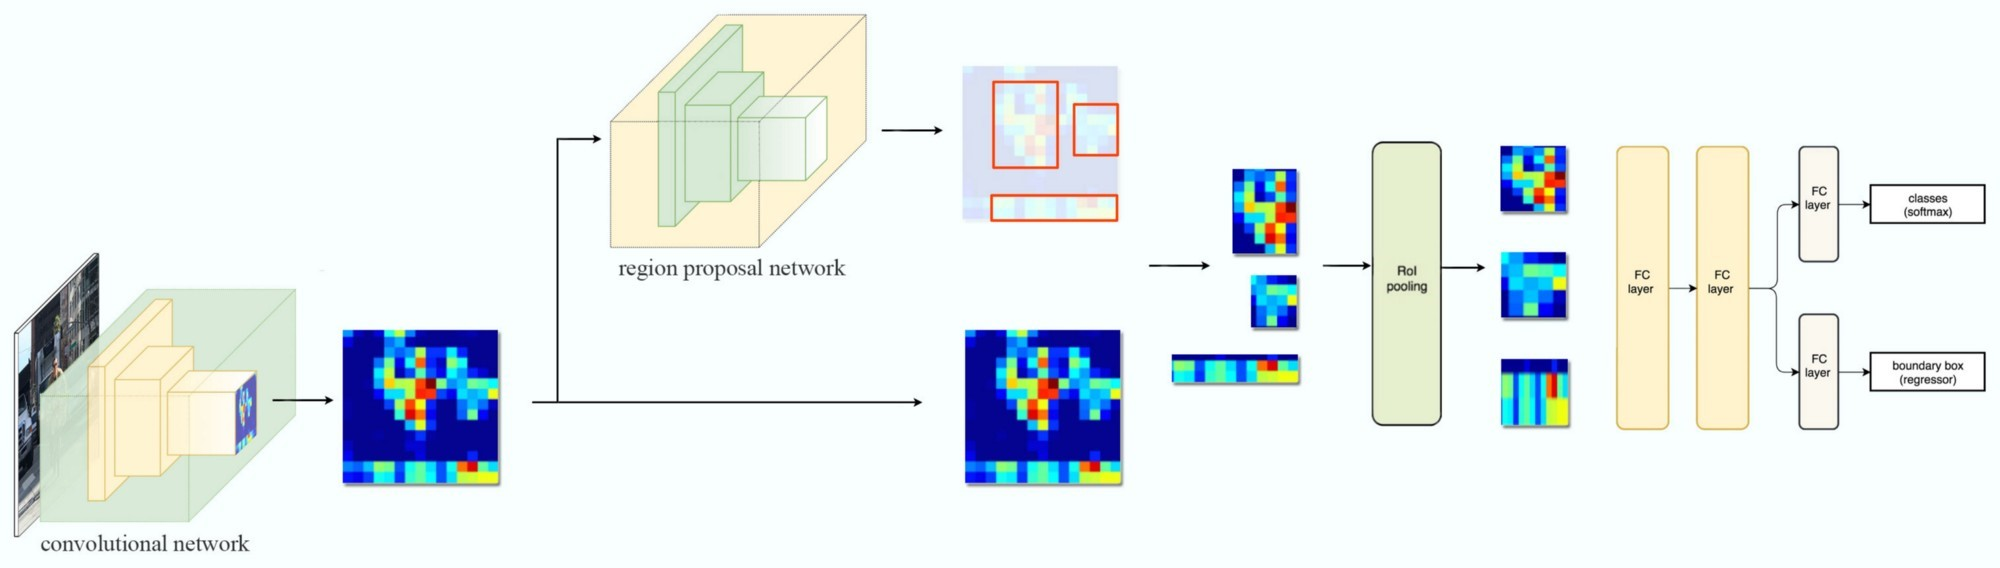
\includegraphics[width=17cm]{man-source/images/ch4/pic4-21.jpg}
	\caption{Глубокая сверточная сеть Faster-RCNN}
	\label{fig:faster_rcnn}
\end{figure}

Такая архитектура обеспечивает получение высоких показателей эффективности при решении задач обнаружения объектов в системах, где общее время, затраченное на обработку и вывод результатов, некритично \cite{Golovko2018}.

\subsection{Обучающая выборка}
Исходными данными, используемыми для формирования обучающей выборки при решении задачи обнаружения солнечных панелей, являлись цветные изображения, полученные из приложения Google Maps с разрешением 200 Х 200 пикселей (рисунок \ref{fig:google_maps}).

\begin{figure}[ht]
	\centering
	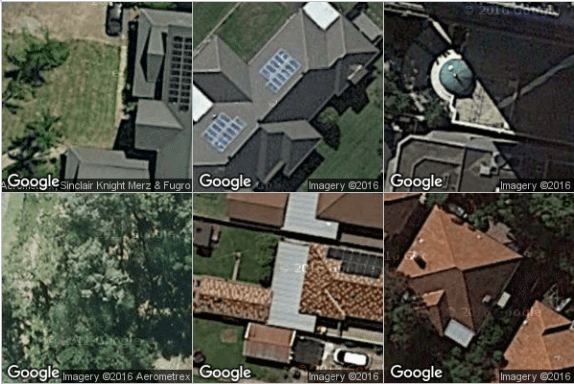
\includegraphics[width=12cm]{man-source/images/ch4/pic4-17.png}
	\caption{Примеры изображений из обучающей выборки}
	\label{fig:google_maps}
\end{figure}

Для обучения модели классификатора использовалась выборка из 3347 фотографий (где 1643 изображения содержали солнечные панели, а 1704 -- не содержали), при этом 80\% исходной выборки формировали обучающую выборку, а 20\% - тестовую. Для обучения модели детектора использовалась выборка из 1000 изображений, 800 из которых было отнесено к обучающей, а 200 -- к тестовой выборкам.

Подготовка обучающей выборки для классификатора состояла в ручном переборе изображений и отнесении их к двум группам изображений -- содержащих солнечные панели и, соответственно, не содержащих. При подготовке обучающей выборки для детектора панелей также использовался ручной перебор изображений с определением для каждого характеристик прямоугольных областей, включающих солнечные панели (длина, ширина, координаты левого верхнего угла). При этом фиксировались все интересующие объекты (для случая множественных панелей). 

Выделение прямоугольных областей для некоторых изображений может не выглядеть целесообразным, например, случаи, когда панели расположены под углом к горизонтальной оси снимка и имеют вытянутую форму (рисунок \ref{fig:background_dominate}). Однако, для таких фотографий удается получить приемлемые результаты локализации на тестовых данных, несмотря на то, что большая часть области включает фоновое изображение.
 
\begin{figure}[ht]
	\centering
	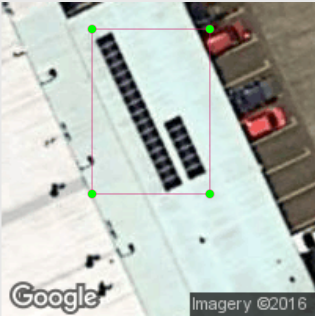
\includegraphics[width=8cm]{man-source/images/ch4/pic4-18.png}
	\caption{Пример изображения с преобладающим фоном}
	\label{fig:background_dominate}
\end{figure}

\subsection{Оценка качества обученных моделей}

Для оценки качества применялись две основные метрики. 

Первая метрика использовалась для оценки классификатора. В режиме тестирования модели применялось простое преобразование выходных данных -- пороговая функция вида:

\begin{equation*}
    b_s = [y_s > 0,5],
\end{equation*}
где $y_s$ представляет реальное выходное значение CNN-сети, возвращаемое для $s$-го входного изображения выборки,\\
$b_s$ -- бинаризованная форма, полученная вычислением нотации Айверсона:

\begin{equation*}
    [x] = 
    \begin{cases}
        1, & \text{x is True} \\
        0, & \text{x is False}.
    \end{cases}
\end{equation*}

Метрика оценки рассчитывалась по формулам:

\begin{equation*}
    A = \frac{S}{L} * 100\%,
\end{equation*}

\begin{equation*}
    S = \sum_{s=1}^L I[b_s = e_s],
\end{equation*}
где $e_s$ -- эталонное значение (метка),\\
$L$ -- объем выборки. 

Таким образом, для оценки эффективности модели подсчитывается общий процент верных ответов, которые были получены с ее помощью на тестовой выборке.

Для оценки эффективности модели локализации использовалась метрика mAP.

Метрика mAP является стандартом де-факто метрик, используемых для оценки качества моделей, применяемых для детекции. Эта метрика используется вместе со своими модификацими, вычисленными для различных значений порога IoU. Так как для рассматриваемой задачи существует только один класс объектов, метрика mAP совпадает с AP.

Как известно, точность вычисляется по формуле:

\begin{equation*}
    P = \frac{TP}{TP + FP},
\end{equation*}
где \textit{TP} и \textit{FP} обозначают соответственно число истинно-положительных и ложно-положительных результатов детекции, и, соответственно,\\
\textit{P} определяет долю корректных детекций в общем числе детекций, полученных моделью.

Величина \textit{TP} равна числу спрогнозированных моделью боксов, для каждого из которых значение \textit{IoU}, вычисленное относительно эталонных боксов (\textit{Ground-true box}), превысило некоторый заданный порог (например, 0,5). В этом случае говорят об истинно-положительной детекции. Если было спрогнозированно несколько боксов для одного бокса-эталона, то выбирается один бокс с наибольшим значением \textit{IoU}, а остальные рассматриваются как \textit{FP}.

Среднее по всем изображениям выборки дает величину AP:

\begin{equation*}
    AP = \frac{1}{L} \sum_{i=1}^L \frac{TP_i}{TP_i + FP_i},
\end{equation*}
где \textit{L} -- число изображений в выборке.

\subsection{Результаты обучения и тестирования}

Сверточная сеть для определения наличия солнечных панелей обучалась в течение 70 эпох, используя следующие параметры:

\begin{easylist}
    & скорость обучения -- 0,001;
    & моментный параметр -- 0,9;
    & weight-decay -- 0,0005;
    & размер мини-батча -- 20;
    & вероятность применения dropout для полносвязных слоев -- 0,5.
\end{easylist}

Точность классификации для данной задачи, составила порядка \textbf{87,46\%} (таблица \ref{table:confusion_matrix}).

\begin{table} [H]
  \small
  \caption{Матрица ошибок}\label{table:confusion_matrix}
\begin{tabularx}{\hsize}{| X | X | X | X |}
  \hline
    & Спрогнозировано <<No>> & Спрогнозировано <<Yes>> & Точность,\% \\
    %\cline{2-3}
    \hline
    Ожидалось <<No>> & 325	& 32	& 91\\
    \hline
    Ожидалось <<Yes>>	& 52	& 261	& 83\\
    \hline
    Итого & 377	& 293	& 87\\
    \hline
\end{tabularx}
\end{table}

На рисунке \ref{fig:roc_curve} изображена ROC-кривая, построенная для обученного классификатора.

\begin{figure}[ht]
	\centering
	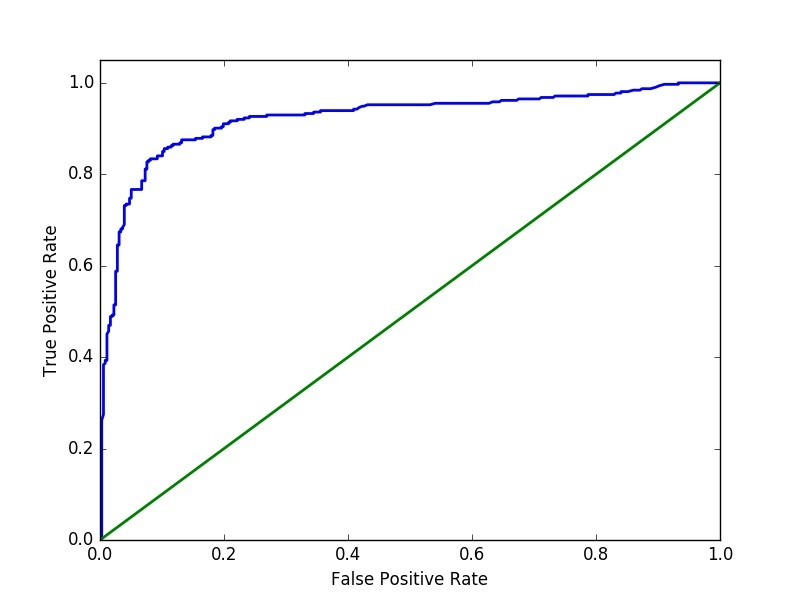
\includegraphics[width=11cm]{man-source/images/ch4/pic4-20.jpg}
	\caption{ROC-кривая для обученного бинарного классификатора, AUC = 0,92}
	\label{fig:roc_curve}
\end{figure}

Другие характеристики полученного классификатора: 
\begin{easylist}
    & полнота = 0,8339, 
    & специфичность = 0,9104, 
    & точность = 0,8907, 
    & F-мера = 0,8614.
\end{easylist}

Сеть для локализации объектов обучалась в течение 5000 итераций (под итерацией здесь понимается настройка параметров для одного случайного изображения из обучающей выборки), используя следующие параметры:

\begin{easylist}
    & скорость обучения -- 0,0003;
    & моментный параметр -- 0,9.
\end{easylist}

После выполнения обучения, проводилось исследование обобщающей способности сети с использованием тестовой выборки из 200 изображений. Полученный результат составил \textbf{\textit{AP}=0,9299}.

Визуализация выходов первого сверточного слоя, полученная после выполнения обучения, представлена на рисунке \ref{fig:pic4-24}.

\begin{figure}[!ht]
	\centering
	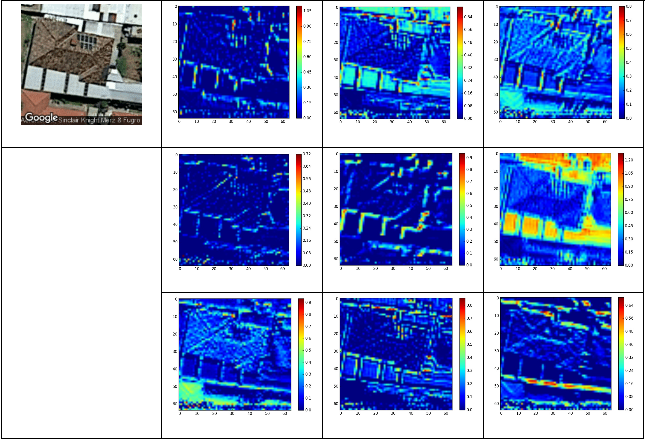
\includegraphics[width=16cm]{man-source/images/ch4/pic4-24.png}
	\caption{Визуализация выходов первого слоя НС}
	\label{fig:pic4-24}
\end{figure}

На рисунке \ref{fig:test_results} изображены результаты детекции солнечных панелей на изображениях из тестовой выборки.

\begin{figure}[!ht]
	\centering
	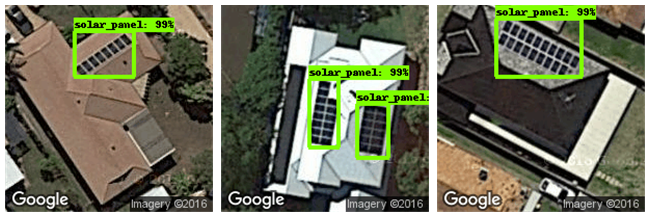
\includegraphics[width=16cm]{man-source/images/ch4/pic4-22.png}
	\caption{Результаты детекции для изображений из тестовой выборки}
	\label{fig:test_results}
\end{figure}

Как можно видеть, предложенный метод осуществляет достаточно точное обнаружение. На рисунке \ref{fig:random_results} изображены результаты работы метода для произвольных изображений (не из тестовой выборки).

\begin{figure}[!ht]
	\centering
	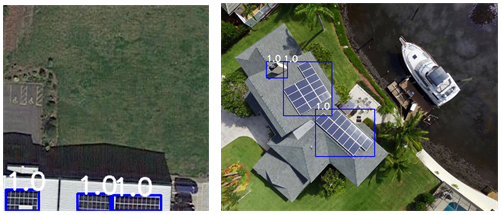
\includegraphics[width=16cm]{man-source/images/ch4/pic4-23.png}
	\caption{Результаты детекции для произвольных изображений}
	\label{fig:random_results}
\end{figure}

\section{Распознавание маркировки продукта}

\subsection{Постановка задачи и обзор существующих решений}

В основе конкурентности любого производства лежит выпуск разнообразной и качественной продукции. Качество является определяющим критерием при выборе клиентом того или иного продукта, а разнообразие позволяет охватить различные группы потенциальных покупателей. Системы, которые автоматизируют процесс проверки качества и при этом поддерживают многообразие продукции, выпускаемой на большом предприятии, имеют особую ценность. При этом процесс проверки качества осуществляется не только для самого продукта, но и для той упаковки и маркировки, которую видит покупатель. Так как упаковка формирует первоначальное впечатление о товаре, ее качество является одной из причин, которая дает покупателю основание для покупки. Маркировка как элемент упаковки, гарантирует покупателю сохранность продукции в течение указанного срока при соблюдении условий хранения.

В последнее время методы искусственного интеллекта в целом и машинного обучения в частности широко используются в промышленных системах, устанавливаемых на предприятиях для контроля за процессом производства. Интеллектуальные подсистемы позволяют упростить многие рутинные операции, проводимые для поддержания качества готовой продукции. Например, контроль за правильностью нанесения маркировки ранее производился исключительно оператором-человеком. Сейчас, с развитием теории компьютерного зрения, получившей значительный рывок благодаря постоянно развивающейся области обучения глубоких нейронных сетей, становится особенно актуальной разработка систем, позволяющих осуществлять рутинные операции быстрее и регулярнее, чем это мог бы сделать человек.

Поставленная задача заключалась в разработке системы распознавания маркировки продуктов, производимых ОАО <<Савушкин продукт>>. Пример продукта с маркировкой, распознавание которой выполняется, представлен на рисунке \ref{fig:digital_code}.

\begin{figure}[ht]
	\centering
	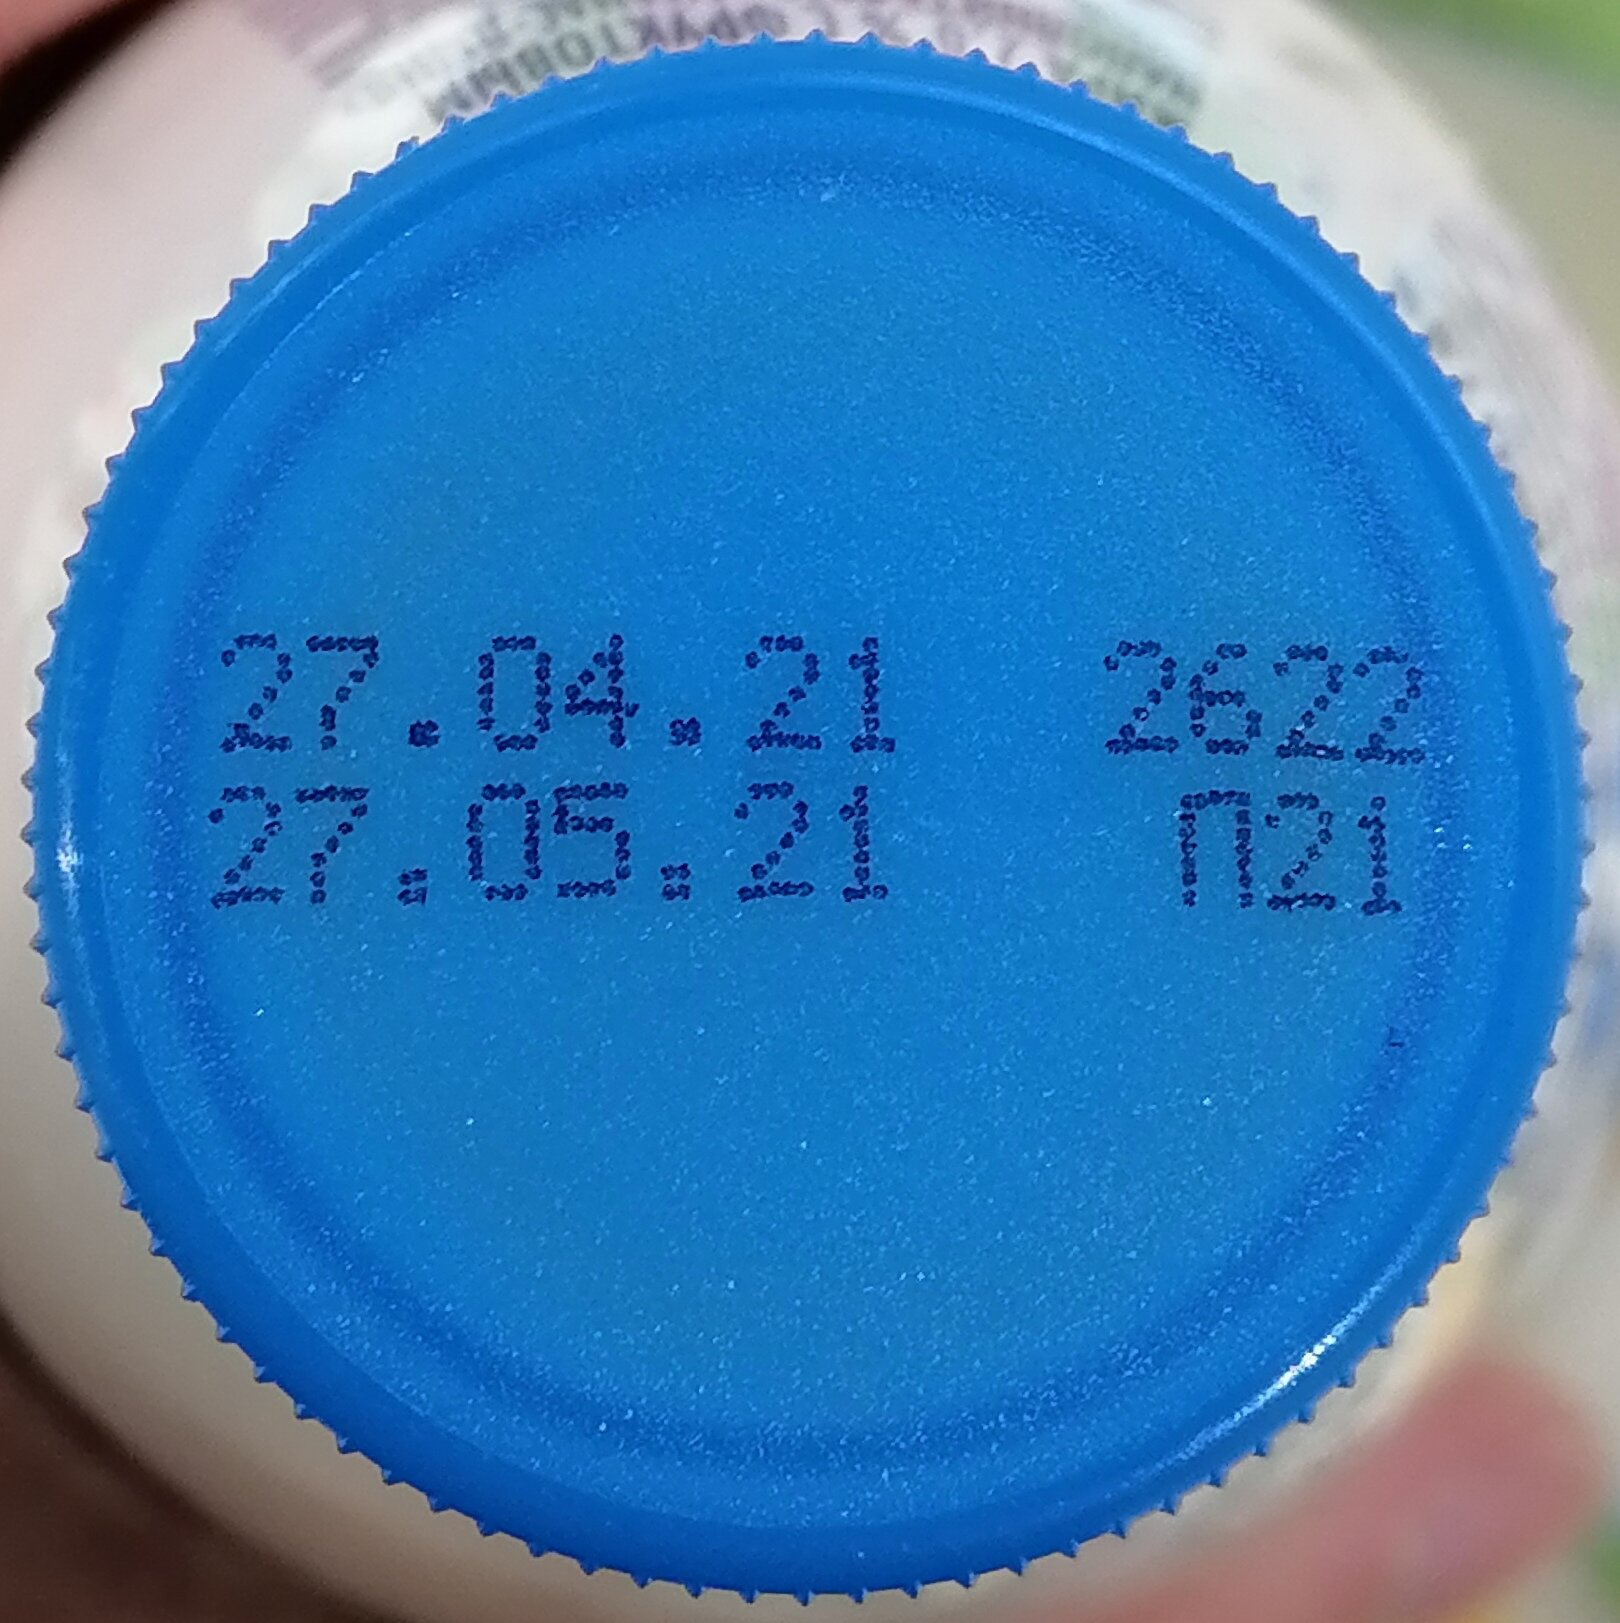
\includegraphics[width=6cm]{man-source/images/ch4/pic4-1.jpg}
	\caption{Продукт с алфавитно-цифровой маркировкой}
	\label{fig:digital_code}
\end{figure}

Важным аспектом является то, что распознавание должно выполняться в реальном времени, основываясь на данных, поступающих с камеры, установленной над производственной линией. Результаты производимого распознавания используются для контроля корректности маркировки.

% Помимо буквенно-цифрового кода (рис. \ref{fig:digital_code}), начиная с недавнего времени, продукция может выпускаться с вариантами маркировки, включающей код Data Matrix (рис. \ref{fig:data_matrix}) \cite{milk}. Данный тип маркировки является удобным и емким представлением специальных и общих данных о продукте. 

% \begin{figure}[ht]
% 	\centering
% 	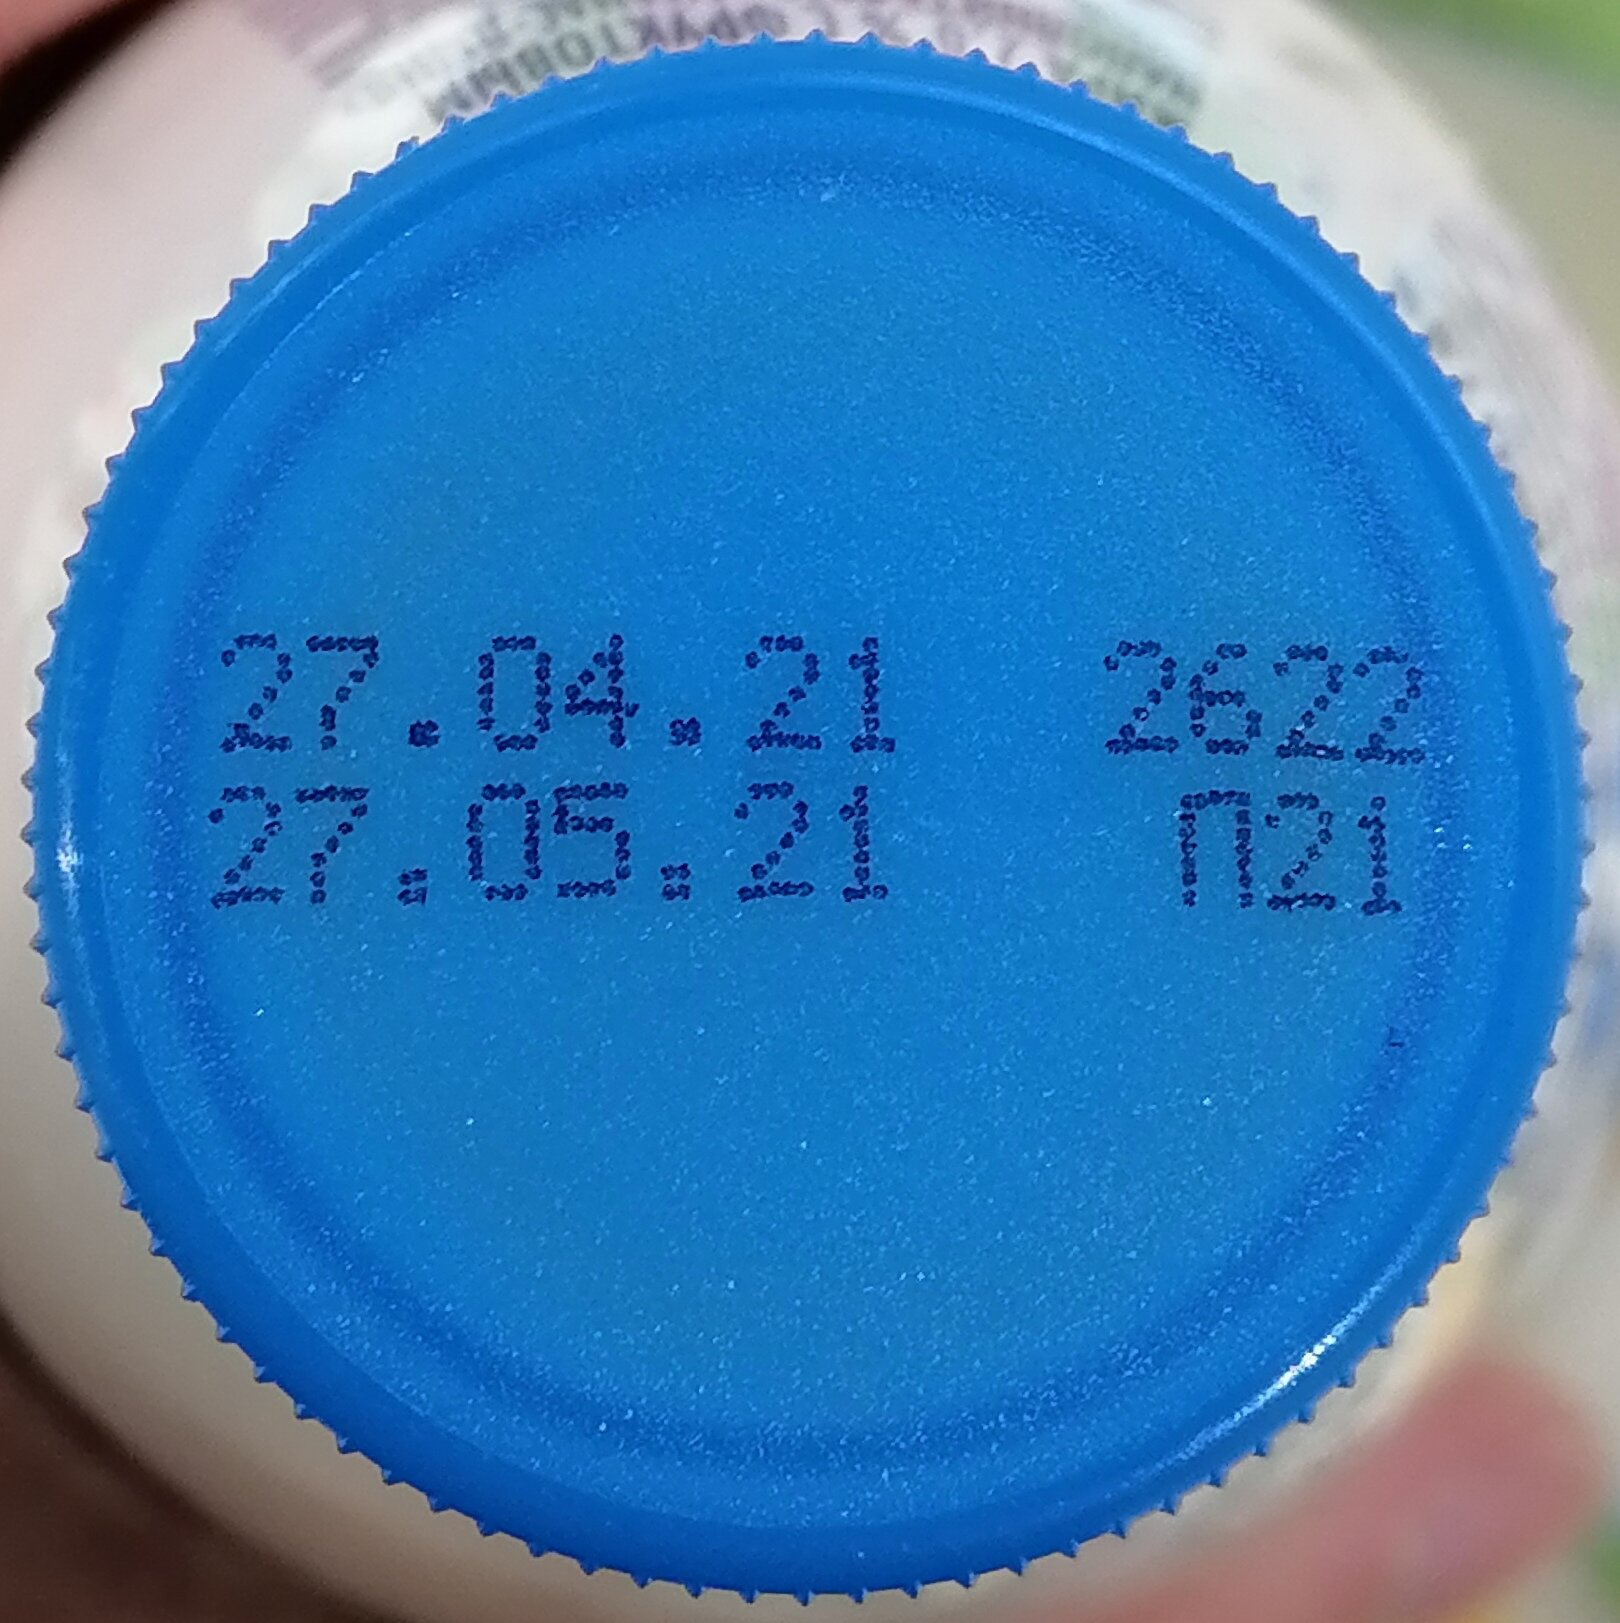
\includegraphics[width=6cm]{man-source/images/ch4/pic4-1.jpg}
% 	\caption{Продукт с буквенно-цифровой маркировкой}
% 	\label{fig:digital_code}
% \end{figure}

% \begin{figure}[ht]
% 	\centering
% 	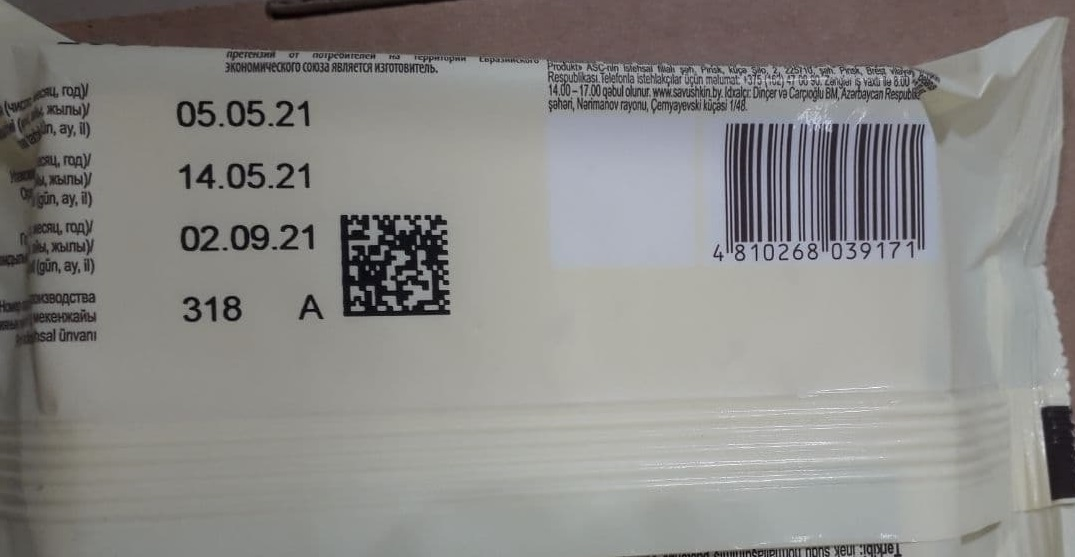
\includegraphics[width=10cm]{man-source/images/ch4/pic4-2.jpg}
% 	\caption{Продукт с кодом Data Matrix}
% 	\label{fig:data_matrix}
% \end{figure}

% Основываясь на общей постановке задачи, были выделены следующие подзадачи, которые должна решать система:
% \begin{easylistNum}
%     & обнаружение и распознавание типа маркировки;
%     & распознавание маркировки;
%     & выявление возможных проблем с маркировкой.
% \end{easylistNum}

К основным проблемам, которые могут возникать в процессе маркирования продуктов, относятся \cite{26-A}:

\begin{easylistNum}
    & \textbf{отсутствие чернил:} в случае поступления на конвейер продуктов без маркировки, система должна сделать вывод об отсутствии чернил, опционально запросив проверку, обратившись к принтеру;
    & \textbf{сдвиг камеры:} если от нейросетевых модулей не поступают данные о результатах распознавания, но системе известно, что движение по конвейеру началось, то она должна сделать вывод о сдвиге камеры;
    & \textbf{ошибочная маркировка:} маркировка была обнаружена и распознана, но не совпала с эталонным представлением. В этом случае должен быть сделан вывод о том, что маркировка неверная;
    & \textbf{нечитаемая маркировка:} в случае, если маркировка получается смазанной и не может быть распознана, необходимо остановить конвейер и сообщить об ошибке оператору.
\end{easylistNum}

Для 1,3 и 4 проблемы необходимо выполнить отсев продуктов, которые имеют ``проблемную'' маркировку. Возникновение этих проблем предполагает полную остановку движения конвейера и сообщение оператору о возникшей проблеме.

Следует отметить, что разработанная система является частью более общей системы, которая используется для анализа и обработки указанных проблем в процессе нанесения маркировки. Общая система реализована с использованием отечественной технологии OSTIS \cite{Golenkov2023}.
%Наша задача заключалась в разработке подсистемы компьютерного зрения для распознавания маркировки продукции.

% Таким образом, резюмируя все вышеназванные задачи и возникающие проблемы, перечислим основные требования, которым должна удовлетворять разрабатываемая система:

% \begin{easylist}
%     & \textbf{Высокая скорость работы}. Конвейер движется очень быстро, поэтому распознавание и анализ должны осуществляться с минимальными задержками;
%     & \textbf{Автономность}. Система должна минимизировать участие оператора;
%     & \textbf{Универсальность}. Система должна настраиваться на распознавание маркировки любой продукции;
%     % & \textbf{Адаптируемость}. Система должна работать при любых условиях, возникающих на производстве (например, недостаточность освещения, ошибки персонала и т.д.).
% \end{easylist}

%Помимо отслеживания маркировки одного лишь человекочитаемого типа (например, буквенно-цифрового), модульная реализация подобных систем позволяет провести универсализацию процесса распознавания и легко добавлять подготовленные модели, осуществляющие распознавание новых типов маркировок, к которым, например, можно отнести код Data Matrix. Такой особый тип матричных штрих-кодов позволяет закодировать специальную идентификационную информацию, а также вес, срок годности, номер серии, номер партии и дату изготовления продукта \cite{datamatrix}.
%Предлагаемая работа посвящена разработке нейросетевого компонента, являющегося частью более общей нейросимволической системы, описанной в \cite{golovko2020}.
Несмотря на существующий интерес к автоматизации производственных процессов и неоспоримые преимущества, которые влечет ее внедрение, подобные задачи решаются в большинстве случаев с участием человека. Оператор периодически выборочно проверяет часть продукции. У такого подхода есть недостатки:

\begin{easylist}
    & есть вероятность того, что будет пропущен момент, когда появится дефект маркировки;
    & скорость реакции человека на возникающую нештатную ситуацию может быть недостаточной;
    & человек может не заметить небольшое расхождение проверяемой маркировки с эталонной (например, в случае ошибочной цифры в дате или номере партии);
    & работа по ручной проверке является монотонной.
\end{easylist}

Существующие аппаратные разработки базируются на использовании специальных датчиков \cite{omron}.

Такие решения осуществляют распознавание маркировки, но имеют ряд важных недостатков:

\begin{easylist}
	& нестабильное качество распознавания, зависящее от условий, при которых производится съемка (в частности, от освещенности). Так как производственная линия движется быстро, то необходимые условия для качественного распознавания чаще всего не соблюдаются;
	& необходимость покупки специализированного программного обеспечения для настройки датчиков.
\end{easylist}

Таким образом, появляется необходимость осуществлять контроль за функционированием самой системы распознавания.

В процессе решения указанной задачи были определены факторы, имеющие критическое влияние на процесс решения и подбор алгоритмов:

\begin{easylist}
	& \textbf{высокая скорость видеопотока}. Так как скорость видеопотока составляет 76 кадров в секунду, то время обработки каждого кадра составляет около 13 миллисекунд. Следует отметить, что этого времени недостаточно для запуска сложной нейросетевой архитектуры, а также для обработки каждого кадра потока;
	& \textbf{сложность корректной прямой детекции символов (цифр)}. Помимо символов, содержащихся непосредственно в маркировке, в кадр могут попадать символы, нанесенные на другие объекты, например, на сам конвейер или его части. Помимо этого, следует отметить, что изображение попадает на нейронную сеть с уменьшенным разрешением, что приводит к сложности распознавания очень мелких объектов.
\end{easylist}

\subsection{Предлагаемый подход}

Предлагаемый подход состоит в использовании конвейерной структуры из отдельных нейросетевых модулей, каждый из которых решает собственную подзадачу распознавания маркировки.

Задачей данного данного конвейера является обнаружение маркировки, определение ее типа и ее распознавание.

Остановимся далее подробнее на архитектуре системы.

Осуществляя декомпозицию решаемой задачи можно выделить следующие подзадачи:

\begin{easylistNum}
	& оценка положения товара;
	& детекция продукта и маркировки;
	& распознавание частей маркировки;
	& <<сборка>> маркировки: формирование выходной информации (даты производства товара, номера в партии и т.д.);
	& проверка распознанной маркировки (определение корректности распознанных данных в соответствии с определенным шаблоном).
\end{easylistNum}

В процессе распознавания маркировки решаются некоторые дополнительные задачи, заключающиеся в проверке корректности печати:

\begin{easylistNum}
    & определение отсутствия маркировки на продукте;
    & определение присутствия искажений маркировки (отсутствия ее частей).
\end{easylistNum}

Указанные задачи решаются в процессе выполнения основных этапов распознавания.

Проблемы, указанные в постановке задачи, решаются архитектурно.

\begin{easylistNum}
    & высокая скорость видеопотока: решается пропуском незначащих кадров, в которых товар находится не в середине кадра. Это позволяет увеличить интервал времени, необходимый для обработки изображения нейросетью. Оценка значимости осуществляется простой моделью-классификатором с малым временем отработки;
    & сложность корректной прямой детекции символов: решается осуществлением декомпозиции задачи обнаружения на отдельные подзадачи. В предлагаемой системе в начале обнаруживается товар, затем маркировка на товаре и, наконец, отдельные символы (цифры).
\end{easylistNum}

В предлагаемой нейросетевой системе практически для каждой подзадачи используется отдельная нейросетевая модель, что позволяет легко модифицировать систему, улучшать отдельные модули, изменять их, а также добавлять новые. 

Архитектура системы распознавания представлена на рисунке \ref{fig:structure}.

\begin{figure}[!ht]
	\centering
	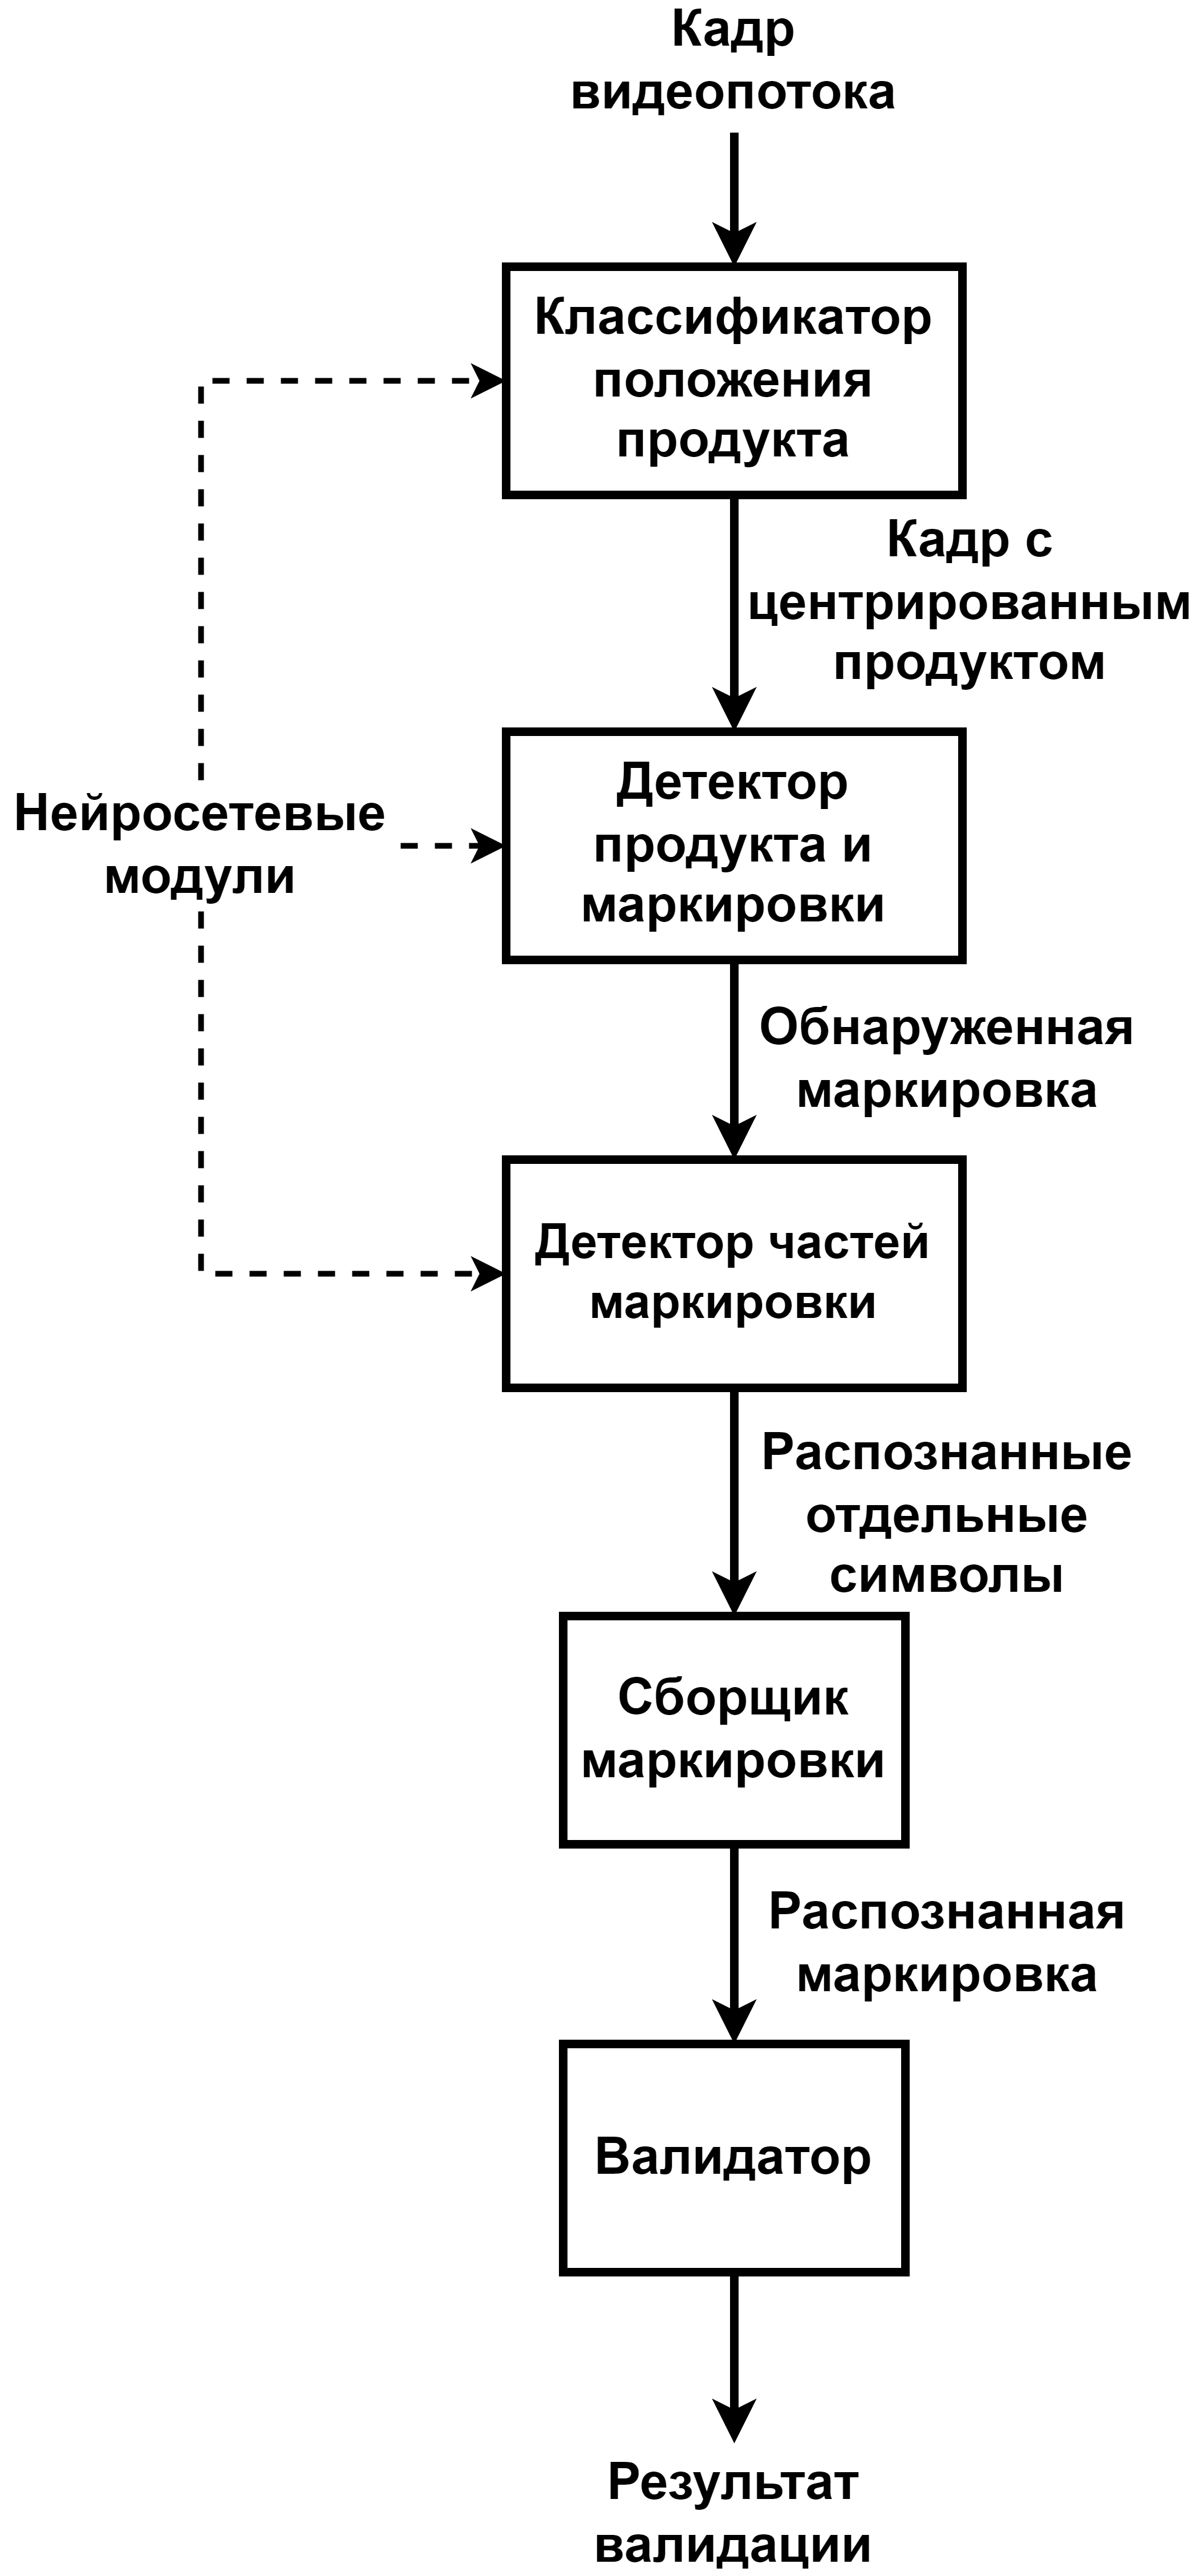
\includegraphics[width=8cm]{man-source/images/ch4/savushkin_structure.png}
	\caption{Структура системы распознавания маркировки}
	\label{fig:structure}
\end{figure}

Опишем основные применяемые нейросетевые модели и их роль в общей архитектуре.

\textbf{Классификатор положения продукта.} Используется предобучаемый сверточный классификатор, который определяет значимость текущего кадра для возможности проведения последующего анализа. При этом наиболее значимым является кадр, в котором товар находится ближе всего к центру кадра (рисунок \ref{fig:distance_classes}). Было выделено 4 класса, представляющих основные позиции продукта в кадре. Класс 1 описывает минимальную удаленность продукта от центра кадра. Кадры, отнесенные к этому классу отбираются для последующих этапов обработки и анализа. Классы 2 и 3 описывают разные степени удаленности (условно среднюю и максимальную). Класс 4 используется для случая отсутствия продукта в кадре (пустая производственная линия).
Кадры, которые идентифицированы как принадлежащие классам 2-4, в дальнейшем анализе не участвуют. 

\begin{figure}[ht]
	\centering
	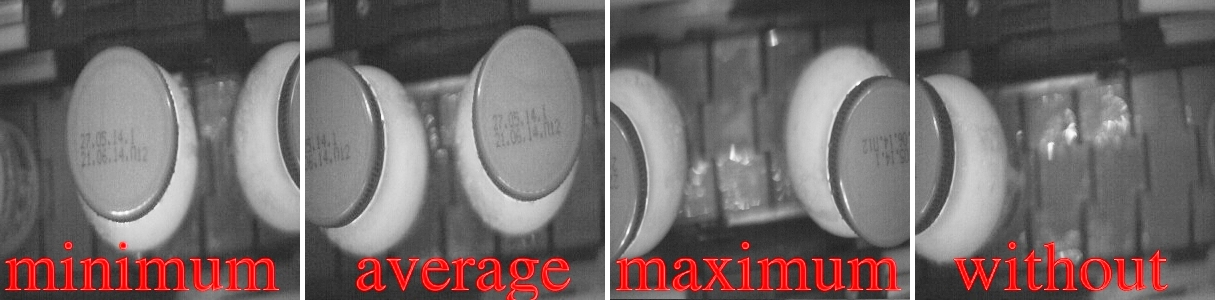
\includegraphics[width=16cm]{man-source/images/ch4/pic4-24.jpg}
	\caption{Примеры изображений разных классов по степени удаленности объекта от центра кадра}
	\label{fig:distance_classes}
\end{figure}

Архитектура применяемого классификатора представлена на рисунке \ref{fig:nn_class1} \cite{7-A}. Он состоит из 5 слоев и имеет 4 выходных нейрона по числу классов, определяющих положение товара в кадре. На всех слоях используется функция активации ReLU за исключением 3-го и последнего слоев. Они используют линейную и softmax-функции активации соответственно. Также применяется max pooling после первого и второго сверточного слоев с параметром stride, равным 2.

\begin{figure}[ht]
	\centering
	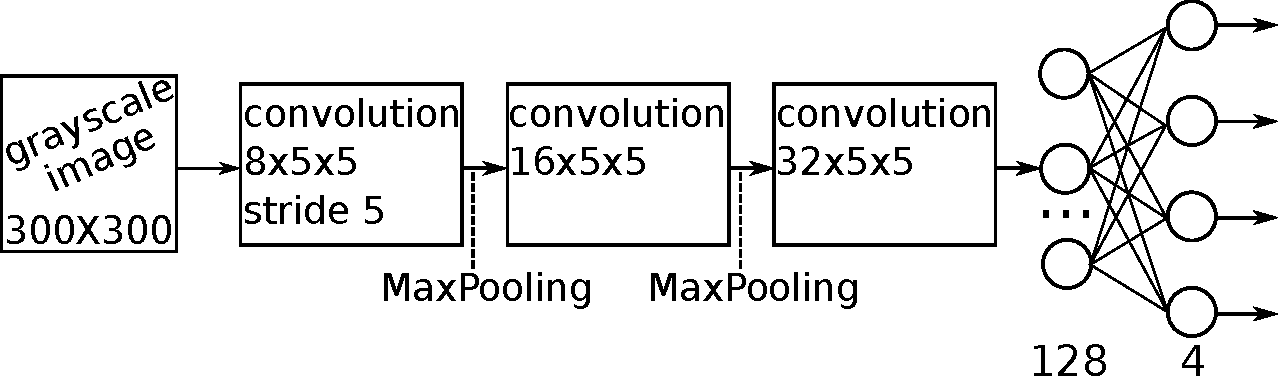
\includegraphics[width=16cm]{man-source/images/ch4/pic4-4.pdf}
	\caption{Структура классификатора для оценки положения бутылки \cite{26-A}}
	\label{fig:nn_class1}
\end{figure}

\textbf{Детектор продукта и маркировки.} Данный детектор осуществляет поиск товара и маркировки в кадре. Здесь в качестве архитектуры была выбрана сеть SSD \cite{liu} на базе классификатора MobileNet v1 \cite{howard}.

Независимое обнаружение товара и маркировки позволяет идентифицировать ситуацию с отсутствующей маркировкой автоматически. Для этого проверяется логическое условие отсутствия маркировки при наличии самого товара в кадре.

Следует отметить, что данный детектор может применяться для обнаружения разных типов маркировки.

В итоге, если маркировка была обнаружена, выполняется передача ее изображения (в оригинальном размере) следующей модели для обработки.

%\textbf{Модуль оценки угла поворота.} В реализации третьего модуля используется регрессор, применяемый для оценки угла поворота маркировки. Данная модель возвращает угол, на который должна быть повернута маркировка для достижения горизонтальной ориентации изображения. Такое преобразование позволяет улучшить качество последующего распознавания цифр. После поворота выполняется передача изображения маркировки на модель для анализа соответствующего типа маркировки (в нашей реализации это модели для анализа кода Data Matrix или цифровой метки).

\textbf{Детектор частей маркировки.} Для анализа алфавитно-цифровой маркировки также используется детектор SSD-MobileNet v1, который осуществляет обнаружение отдельных цифр маркировки.
%Для анализа кода Data Matrix в текущей реализации используется не нейросетевая модель. Применимость нейронной сети для подобного анализа может быть предметом дальнейших исследований.  

После отработки детектора составных частей осуществляется <<сборка>> распознанной маркировки и обработка результата.

Принцип работы нейросетевого компонента на примере алфавитно-цифровой маркировки продемонстрирован на рисунке \ref{fig:system_work}.

\begin{figure}[!ht]
	\centering
	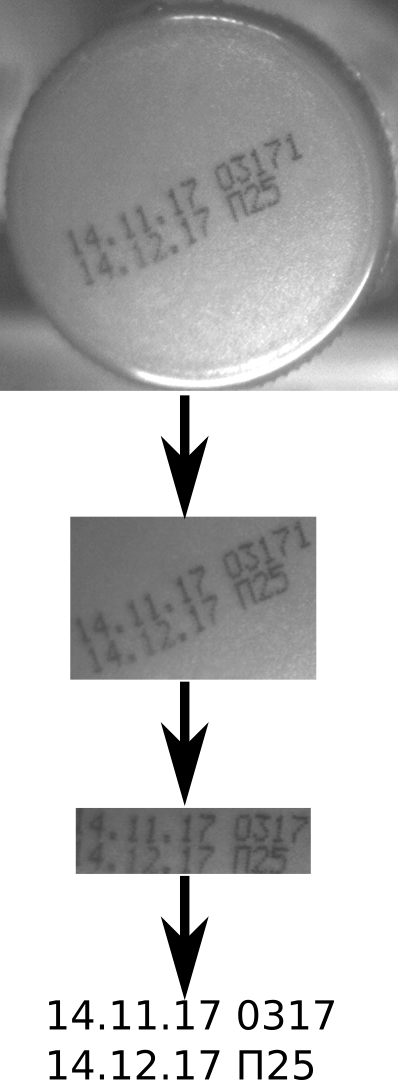
\includegraphics[width=7cm]{man-source/images/ch4/pic4-5.png}
	\caption{Принцип работы системы}
	\label{fig:system_work}
\end{figure}

\subsection{Обучающие выборки}

В процессе подготовки нейросетевых моделей использовались различные обучающие выборки:

\begin{easylist}
	& выборка для обучения классификатора положения;
	& выборка для обучения детектора маркировок и товаров;
	%& Выборка для обучения регрессора угла поворота
	& выборка для обучения детектора частей маркировки.
\end{easylist} 

\textbf{Выборка для обучения классификатора положения продукта}. Для создания выборки использовалась модель Faster R-CNN \cite{ren} (на базе  предобученного классификатора ResNet50 \cite{he}). Данная модель обладает лучшими показателями эффективности, чем SSD-MobileNet, но уступает ей в скорости. Она использовалась для автоматической разметки имеющихся данных (главным образом видеофайлов производственного процесса) по степени удаленности товара от центра кадра. В качестве метрики применялось эвклидово расстояние от центра продукта до центра кадра. Таким образом были сформированы четыре класса изображений, которые использовались для последующего обучения сверточного классификатора. Общий объем выборки составил 6189 изображений, 1303 из которых составили тестовую выборку.

\textbf{Выборка для обучения детектора продукта и маркировки}. Для формирования этой выборки использовались размеченные вручную изображения. Общий объем выборки составил 815 изображений, 163 из которых составили тестовую выборку.

%\textbf{Выборка для обучения регрессора угла поворота}. При создании данной выборки использовались изображения маркировок, повернутые под произвольными углами. Общий объем выборки составил 59385 изображений, 11877 из которых составили контрольную выборку. В качестве основы брались изображения маркировок, полученные из выборки для обучения детектора маркировок и товаров.

\textbf{Выборка для обучения детектора частей маркировки}. Для создания этой выборки применялась выборка SVHN \cite{netzer} (выборка номеров домов), а также размеченные цифровые маркировки из уже сформированных выборок. Использовался вариант выборки SVHN, включающий 33402~изображения в обучающей части и 13068 в тестовой (рисунок \ref{fig:svhn_dataset}). Объем выборки размеченных цифровых маркировок составил 419 изображений.

\begin{figure}[ht]
	\centering
	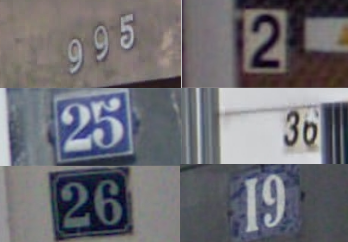
\includegraphics[width=7cm]{man-source/images/ch4/pic4-14.png}
	\caption{Пример изображений из выборки SVHN}
	\label{fig:svhn_dataset}
\end{figure}

\subsection{Результаты обучения и тестирования} 
После обучения классификатора положения продукта итоговая точность распознавания составила \textbf{93.27\%}. Для обучения данной модели применялось предобучение по предлагаемому методу REBA.

Оба детектора (продуктов/маркировок и частей маркировки) обучались на основе предобученных моделей (использовалось предобучение I~типа).

Применение SSD-модели позволило достичь эффективности детекции в \textbf{99\% (mAP = 0.99)} для обнаружения товара и маркировки и \textbf{92\% (mAP = 0.92)} для отдельных цифр. Кроме этого, высокая скорость обработки позволила успешно обнаруживать маркировку в видеопотоке. Результаты эффективности распознавания отдельных цифр представлены в таблице \ref{tab:efficiency_detector1}.  

\begin{table}[h]
\caption{Эффективность обнаружения отдельных классов цифр}
\centering
\begin{tabular}{ | c | c |  }
\hline
Class label & AP \\ \hline
0 & 0.9218\\
1. & 0.9107\\
2. & 0.9354\\
3. & 0.9286\\
4. & 0.9265\\
5. & 0.9137\\
6. & 0.9274\\
7. & 0.9167\\
8. & 0.9646\\
9. & 0.8975\\
\hline
\textbf{mAP} & \textbf{0.92429}\\
\hline
\end{tabular}
\label{tab:efficiency_detector1}
\end{table}

Результаты работы детектора продукта и маркировки и детектора частей маркировки изображены на рисунках \ref{fig:product_detect}  и \ref{fig:numbers_detect}.

\begin{figure}[!ht]
	\centering
	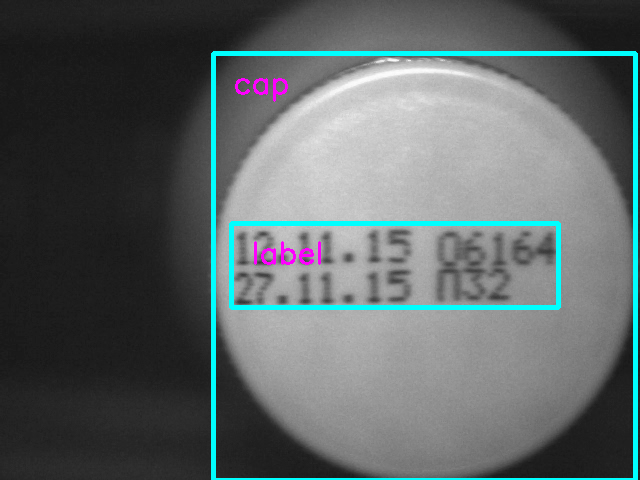
\includegraphics[width=10cm]{man-source/images/ch4/pic4-25.png}
	\caption{Обнаруженный продукт и маркировка}
	\label{fig:product_detect}
\end{figure}

\begin{figure}[!ht]
	\centering
	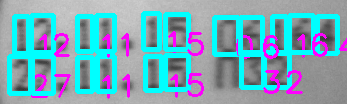
\includegraphics[width=12cm]{man-source/images/ch4/pic4-26.png}
	\caption{Обнаруженные цифры в маркировке}
	\label{fig:numbers_detect}
\end{figure}

Помимо алфавитно-цифровой маркировки (рисунок \ref{fig:digital_code}), начиная с недавнего времени, продукция ООО <<Савушкин Продукт>> выпускается с вариантами маркировки, включающей код Data Matrix (рисунок \ref{fig:data_matrix}) \cite{milk}. Данный тип маркировки является удобным и емким представлением специальных и общих данных о продукте. 

% \begin{figure}[ht]
% 	\centering
% 	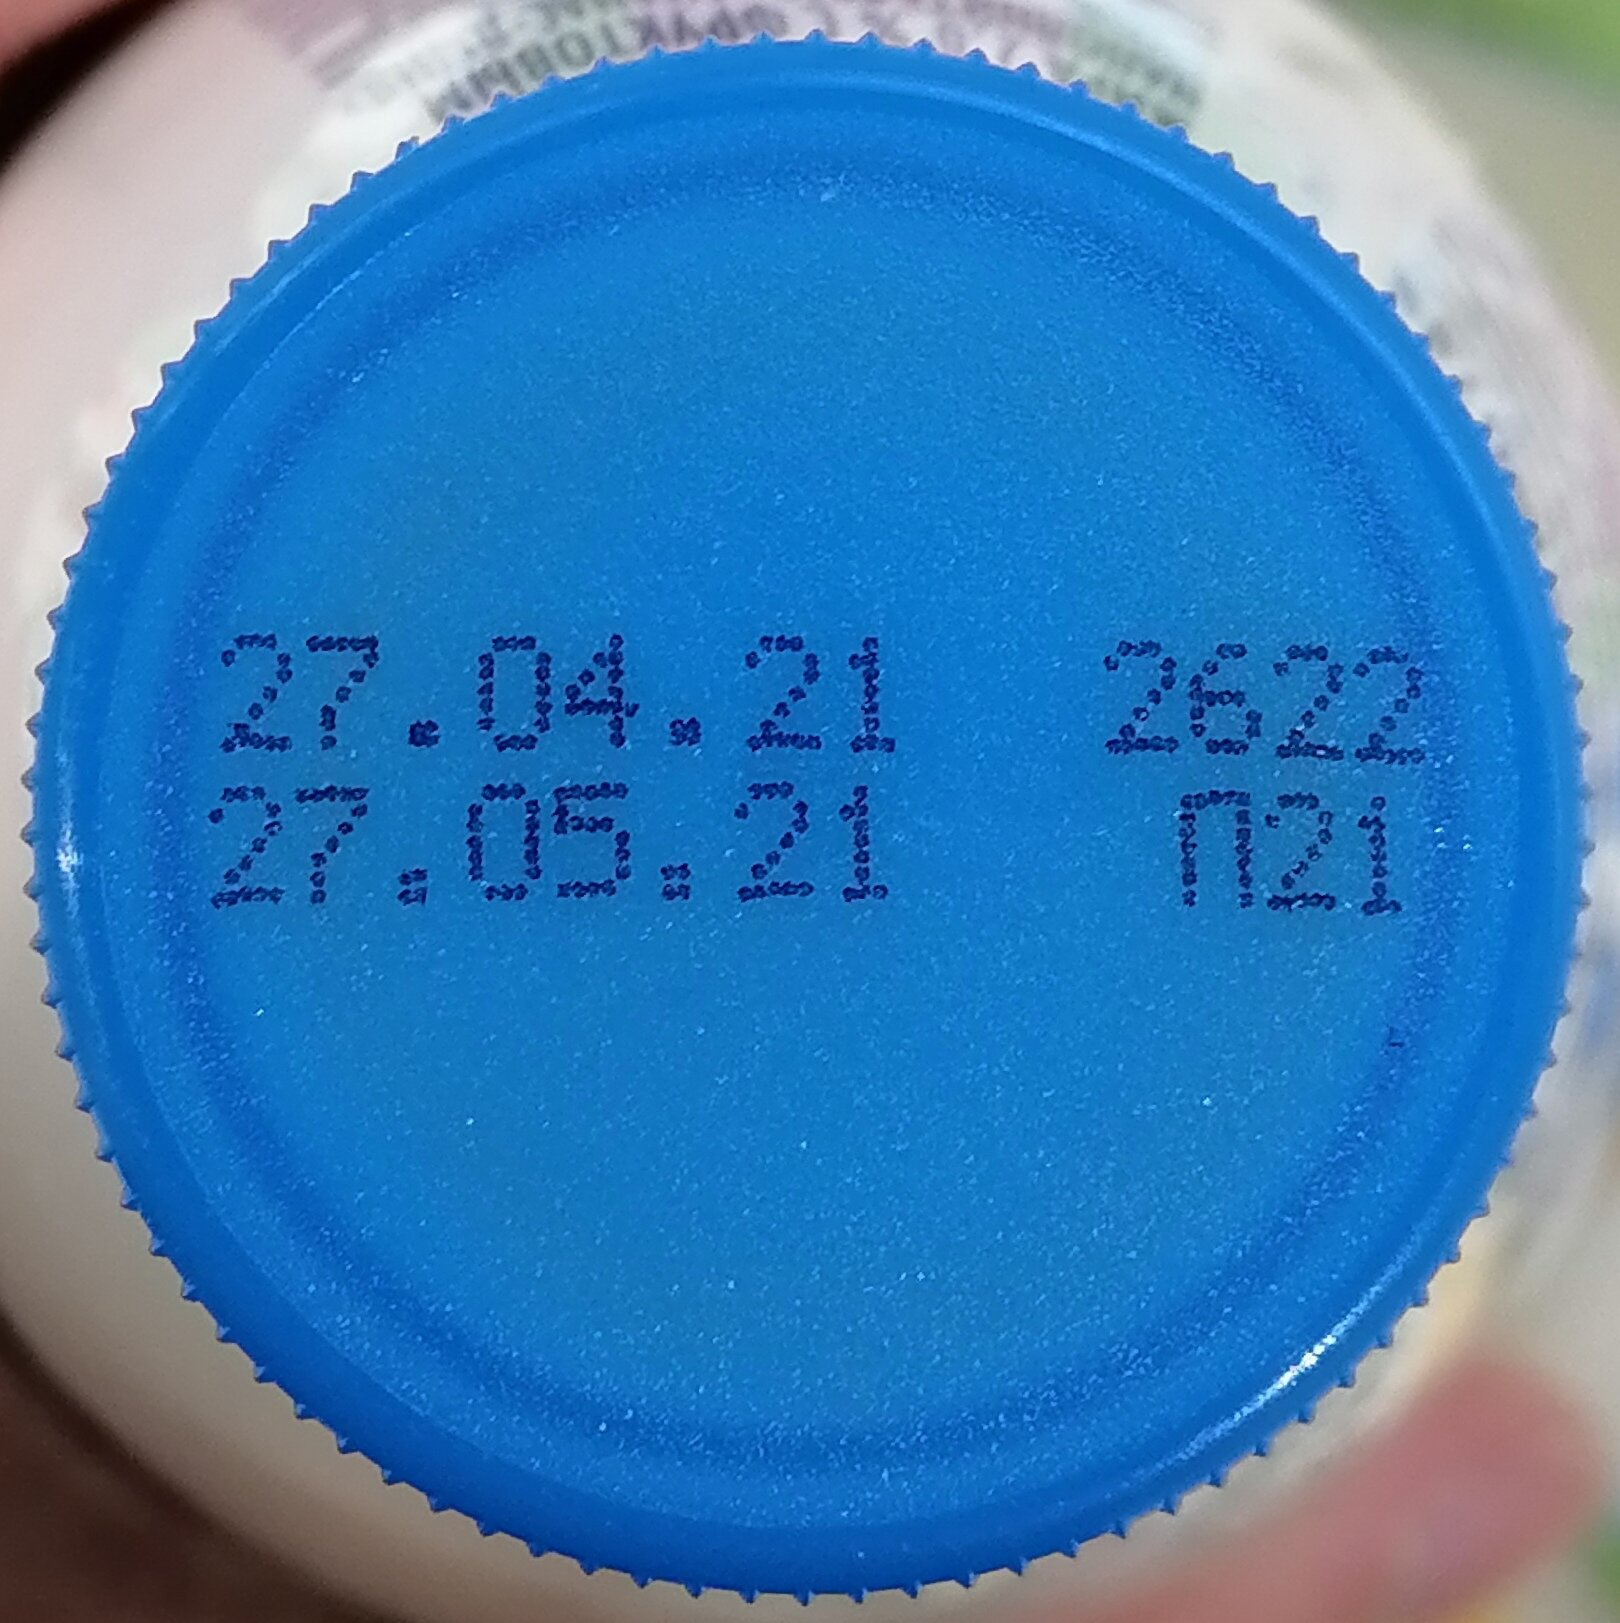
\includegraphics[width=6cm]{man-source/images/ch4/pic4-1.jpg}
% 	\caption{Продукт с буквенно-цифровой маркировкой}
% 	\label{fig:digital_code}
% \end{figure}

\begin{figure}[!ht]
	\centering
	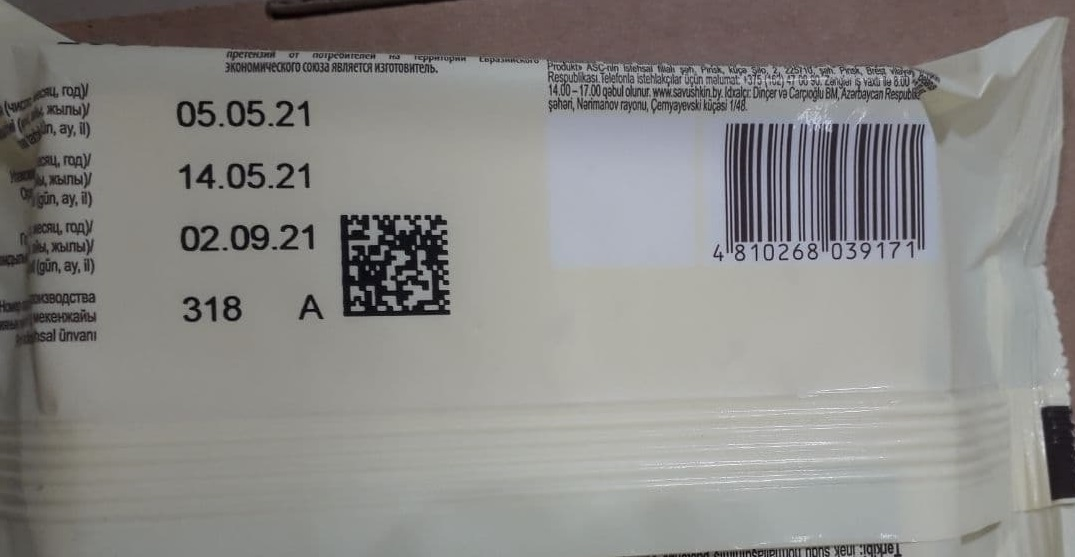
\includegraphics[width=10cm]{man-source/images/ch4/pic4-2.jpg}
	\caption{Продукт с кодом Data Matrix}
	\label{fig:data_matrix}
\end{figure}

Внедрение нового типа маркировки не снижает актуальность предлагаемой разработки, поскольку алфавитно-цифровая маркировка остается единственным вариантом маркировки, который может быть распознан непосредственно человеком. Помимо этого, он продолжает использоваться на всей продукции.

Отметим также, что расширение разработанной системы для обработки новых типов маркировки возможно путем дообучения детектора маркировок на новых данных. Это позволяет гибко расширять систему без необходимости ее повторной реализации.

\section{Выводы}

\begin{easylistNum}
    & Предложено решение задачи определения наличия и детекции солнечных панелей на аэрофотоснимках. Достоинством предлагаемого решения является возможность работы с изображениями, имеющими низкое разрешение. Использование предобученных сверточных нейронных сетей позволило достичь точности 87,46 \% в определении наличия солнечных панелей на фото \cite{9-A, 14-A, 15-A}.
	& Предложено решение задачи распознавания маркировки продукта на производственной линии. Достоинствами предлагаемого решения является модульная структура, позволяющая осуществлять независимую поддержку каждого функционального модуля. Разработанные нейросетевые модули позволили осуществлять оценку положения продукта на изображении с точностью 93.27\%, локализацию маркировки и продукта с точностью 99\% и обнаружение отдельных составляющих маркировки (цифр) с точностью 92\% \cite{7-A, 29-A, 6-A, 25-A, 27-A, 23-A, 24-A, 8-A, 26-A, 28-A}.
\end{easylistNum}
